\section{Sobreajuste y poda}


texto



En la figura~\ref{fig:3a} se muestra la grafica el número de hojas en función de la función de poda.

\begin{figure}
  \centering
  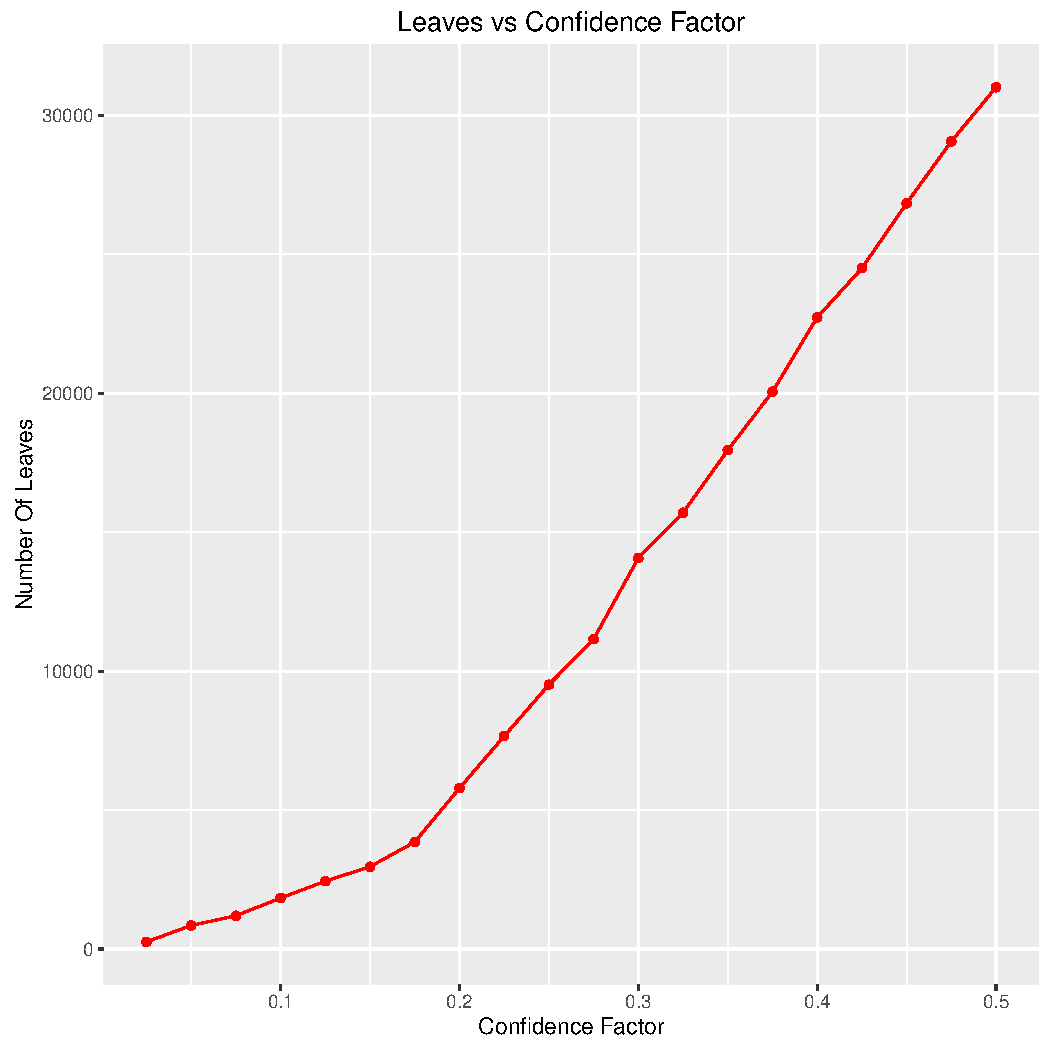
\includegraphics[width = 8cm]{3a.pdf}
  \caption{Number of leaves vs Confidence factor}
  \label{fig:3a}
\end{figure}

En la figura~\ref{fig:3b} se muestra la grafica el performance en función de la función de poda.

\begin{figure}
  \centering
  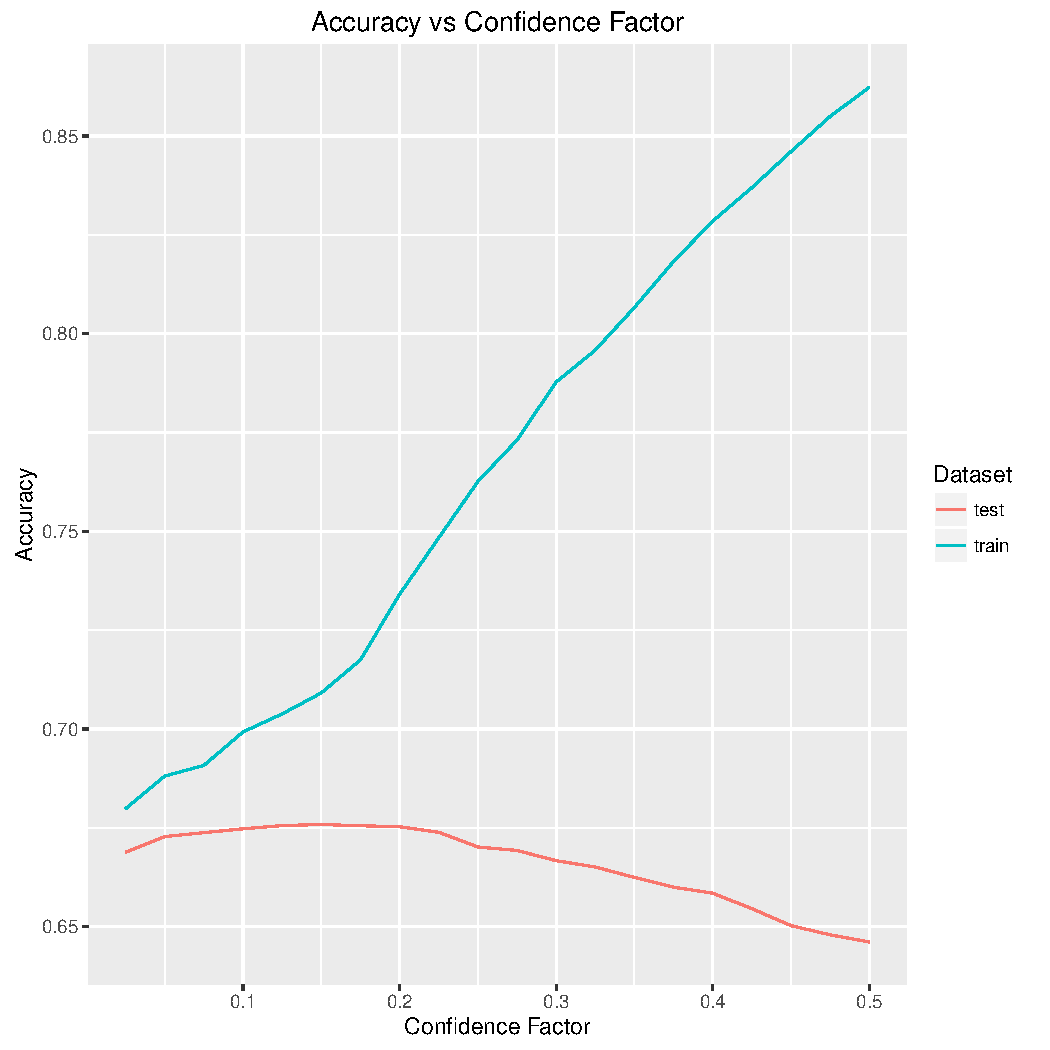
\includegraphics[width = 8cm]{3b.pdf}
  \caption{Accuracy vs Confidence factor}
  \label{fig:3b}
\end{figure}


En la figura~\ref{fig:3c} se muestra la grafica de la curva ROC para el mejor árbol,

\begin{figure}
  \centering
  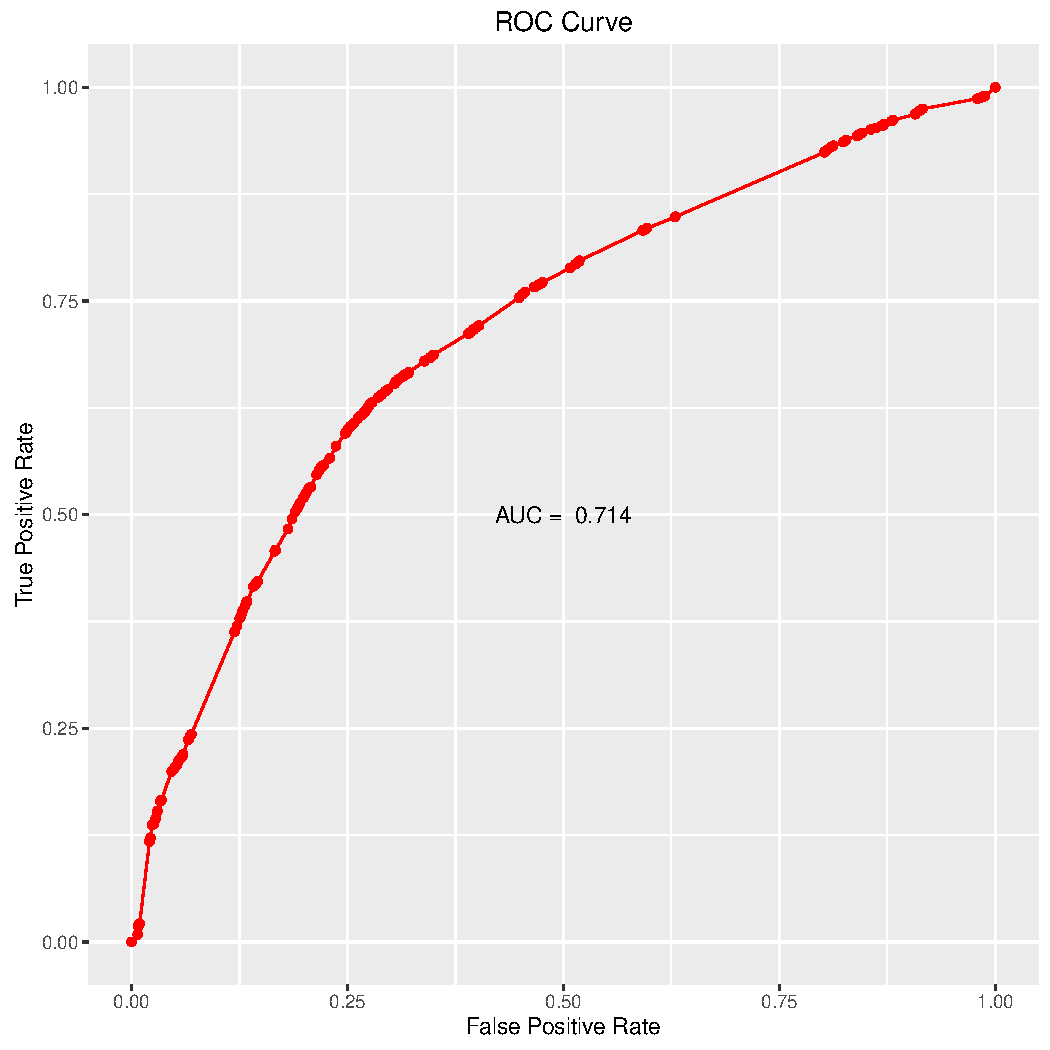
\includegraphics[width = 8cm]{3c.pdf}
  \caption{Curva ROC mejor árbol}
  \label{fig:3c}
\end{figure}

En la figura~\ref{fig:4a} se muestra la grafica de la curva ROC para el mejor árbol,

\begin{figure}
  \centering
  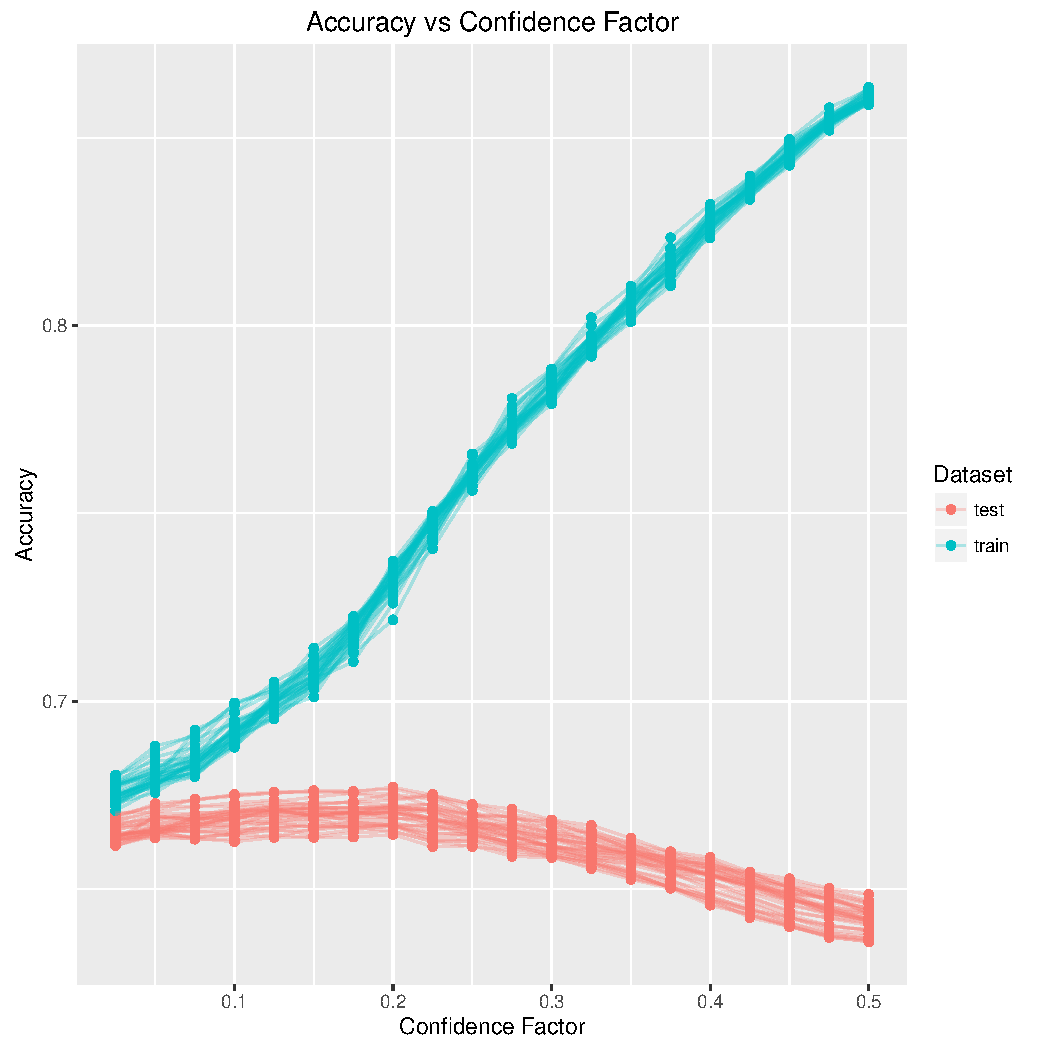
\includegraphics[width = 8cm]{4a.pdf}
  \caption{Accuracy vs Confidence factor with missing data}
  \label{fig:4a}
\end{figure}

En la figura~\ref{fig:4b} se muestra la grafica de la curva ROC para el mejor árbol,

\begin{figure}
  \centering
  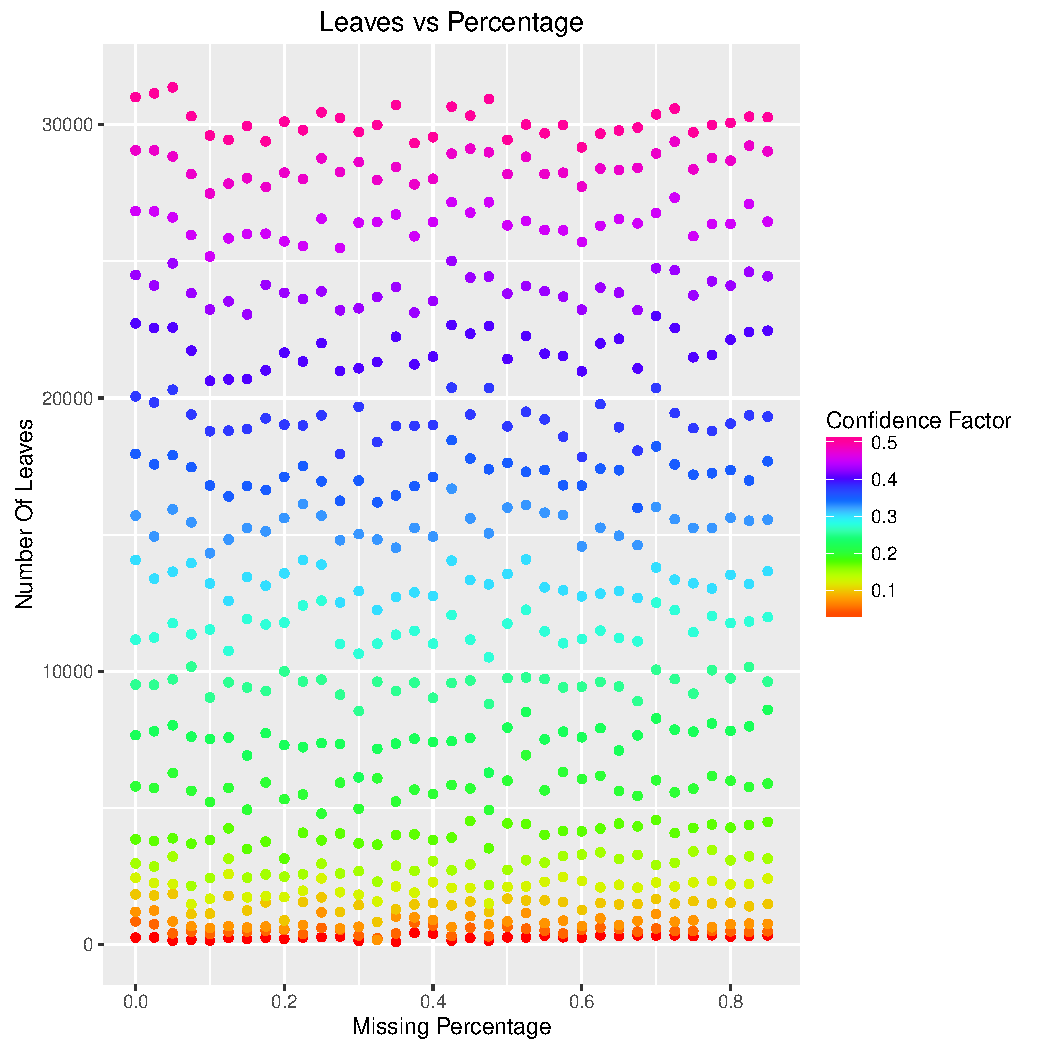
\includegraphics[width = 8cm]{4b.pdf}
  \caption{Leaves vs missing percentage}
  \label{fig:4b}
\end{figure}

En la figura~\ref{fig:4c} se muestra la grafica de la curva ROC para el mejor árbol,

\begin{figure}
  \centering
  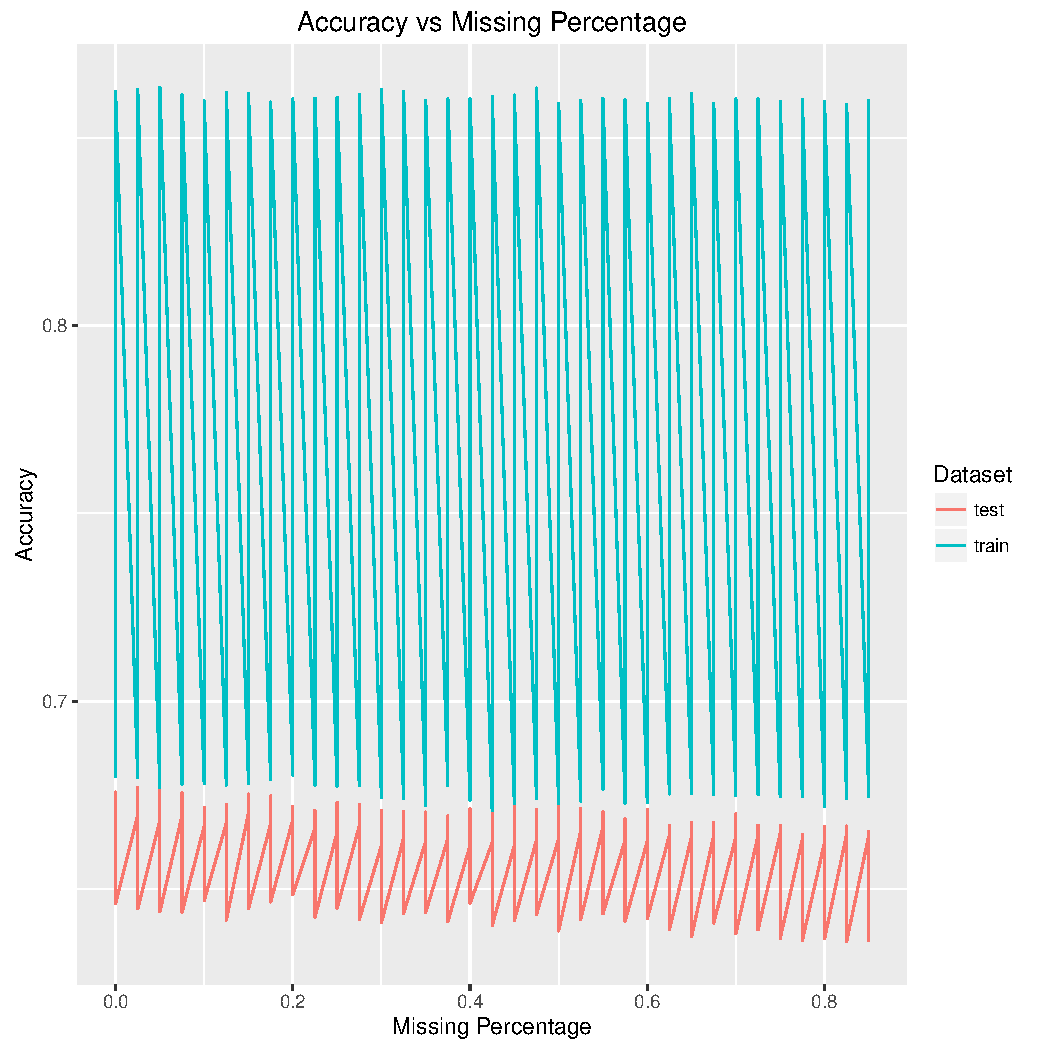
\includegraphics[width = 8cm]{4c.pdf}
  \caption{Accuracy vs missing percentage}
  \label{fig:4c}
\end{figure}

En la figura~\ref{fig:4d} se muestra la grafica de la curva ROC para el mejor árbol,

\begin{figure}
  \centering
  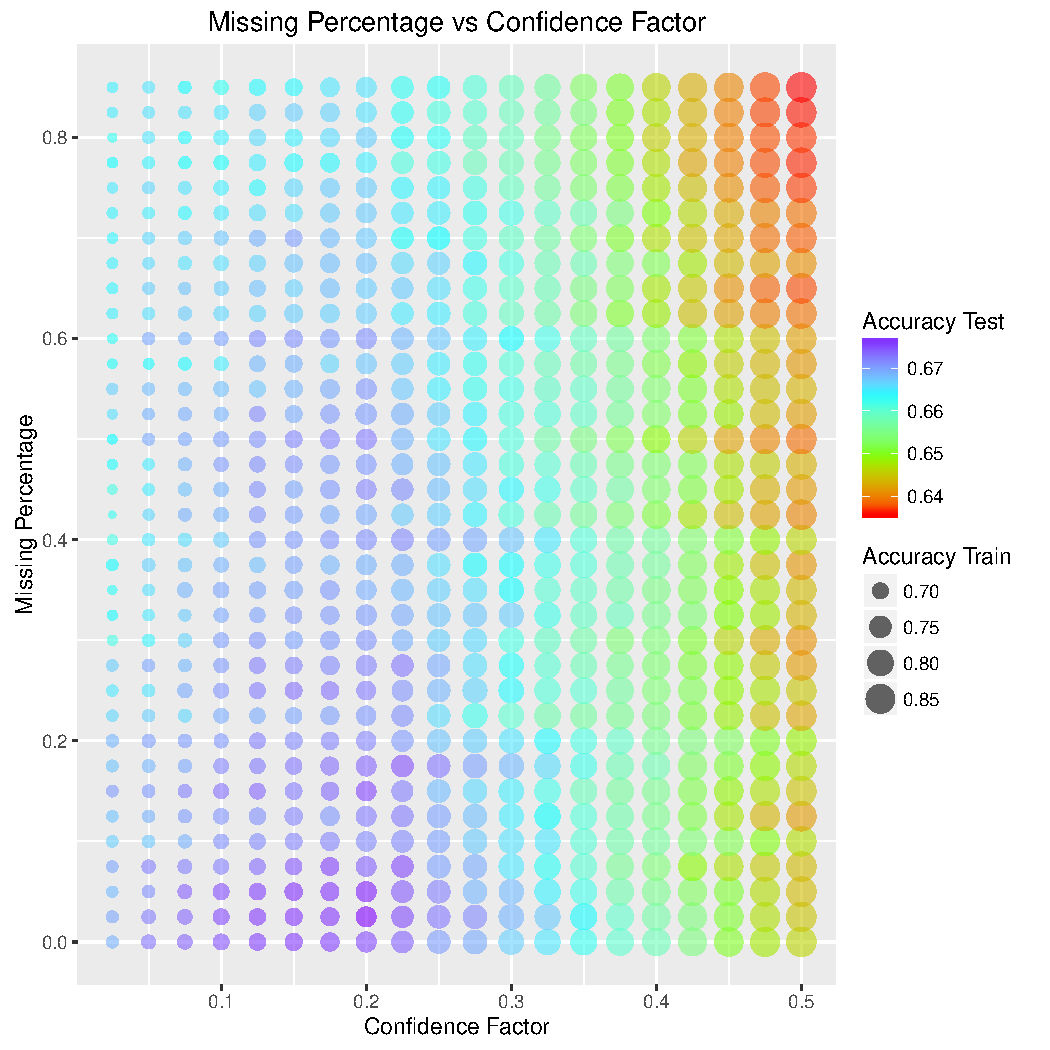
\includegraphics[width = 8cm]{4d.pdf}
  \caption{Missing percentage vs Confidence factor}
  \label{fig:4d}
\end{figure}

En la figura~\ref{fig:5a} se muestra la grafica de la curva ROC para el mejor árbol,

\begin{figure}
  \centering
  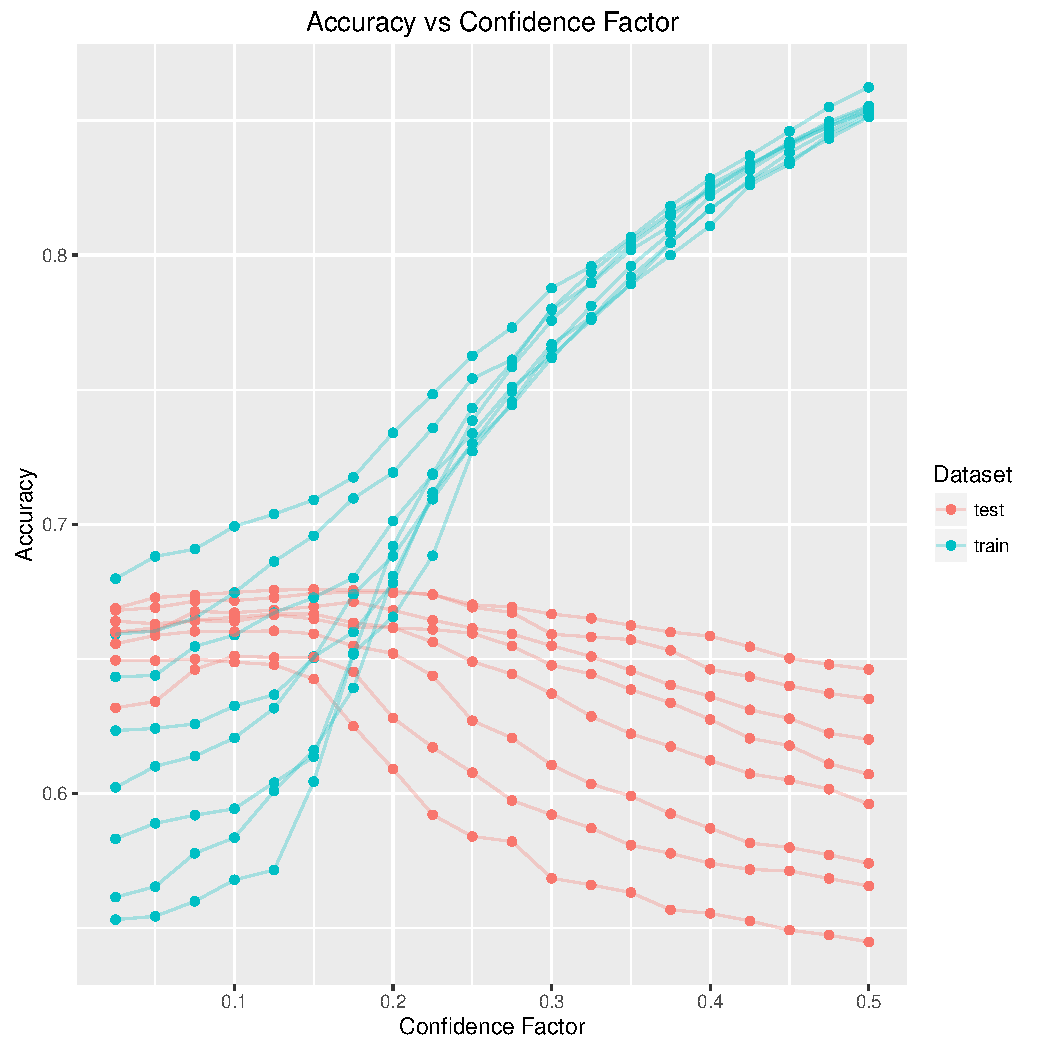
\includegraphics[width = 8cm]{5a.pdf}
  \caption{Accuracy vs Confidence factor with noise data}
  \label{fig:5a}
\end{figure}

En la figura~\ref{fig:5b} se muestra la grafica de la curva ROC para el mejor árbol,

\begin{figure}
  \centering
  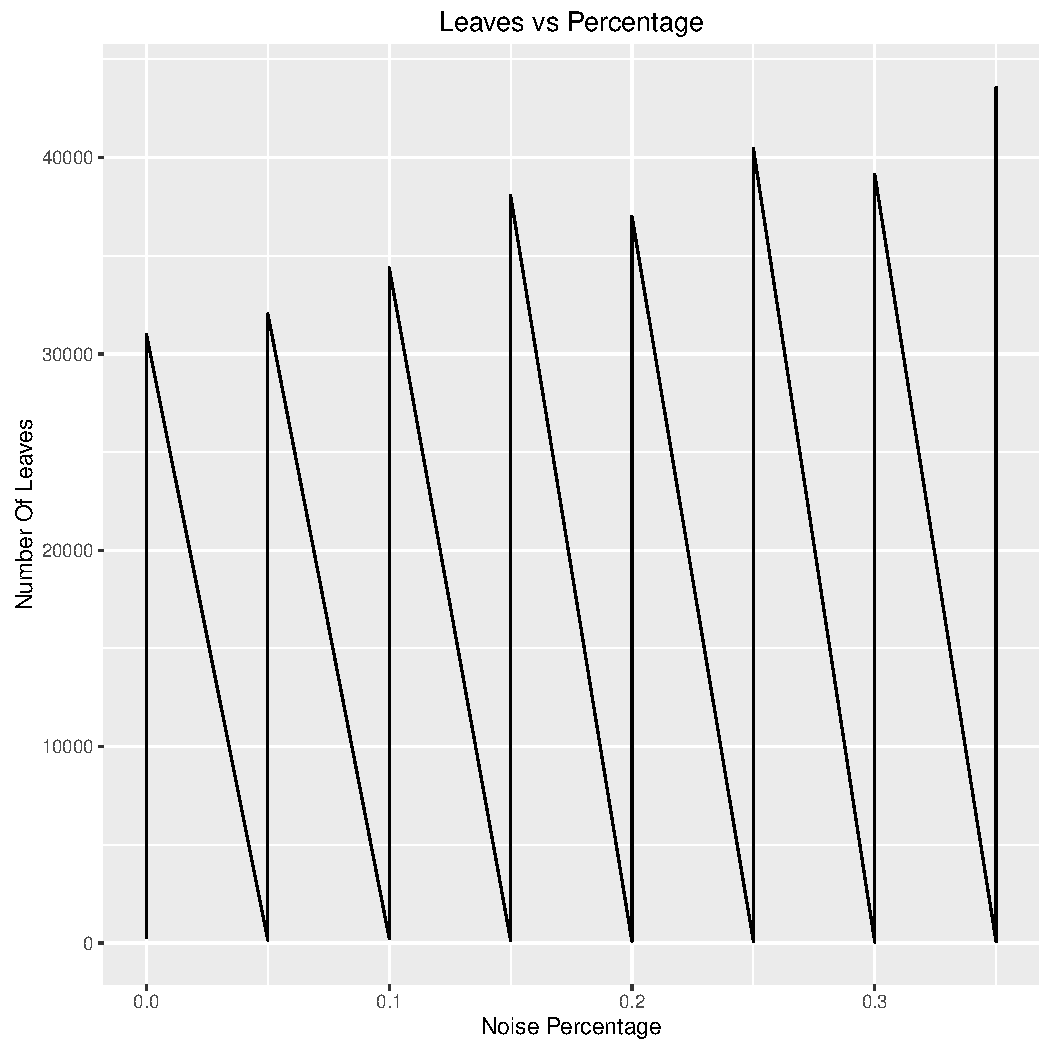
\includegraphics[width = 8cm]{5b.pdf}
  \caption{Leaves vs noice percentage}
  \label{fig:5b}
\end{figure}

En la figura~\ref{fig:5c} se muestra la grafica de la curva ROC para el mejor árbol,

\begin{figure}
  \centering
  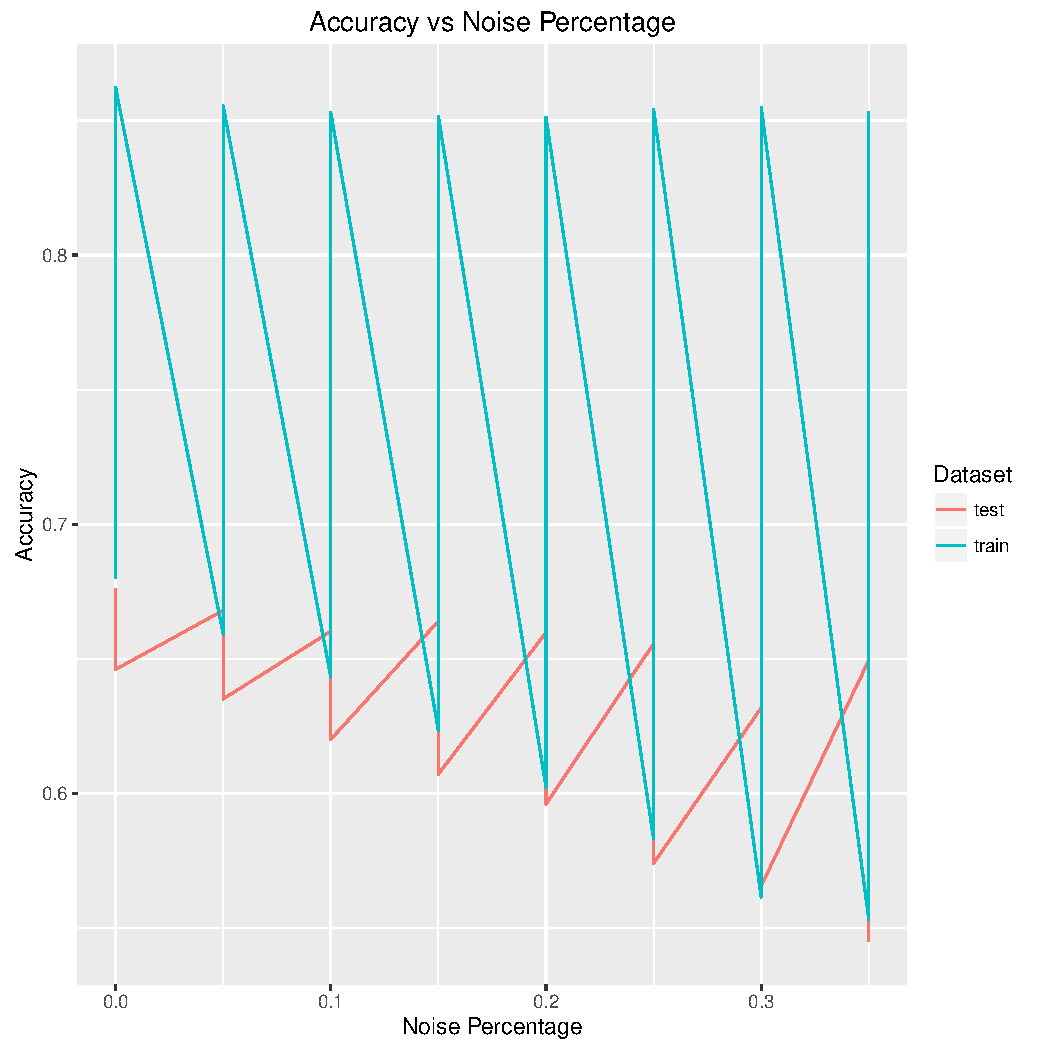
\includegraphics[width = 8cm]{5c.pdf}
  \caption{Accuracy vs noise percentage}
  \label{fig:5c}
\end{figure}

En la figura~\ref{fig:5d} se muestra la grafica de la curva ROC para el mejor árbol,

\begin{figure}
  \centering
  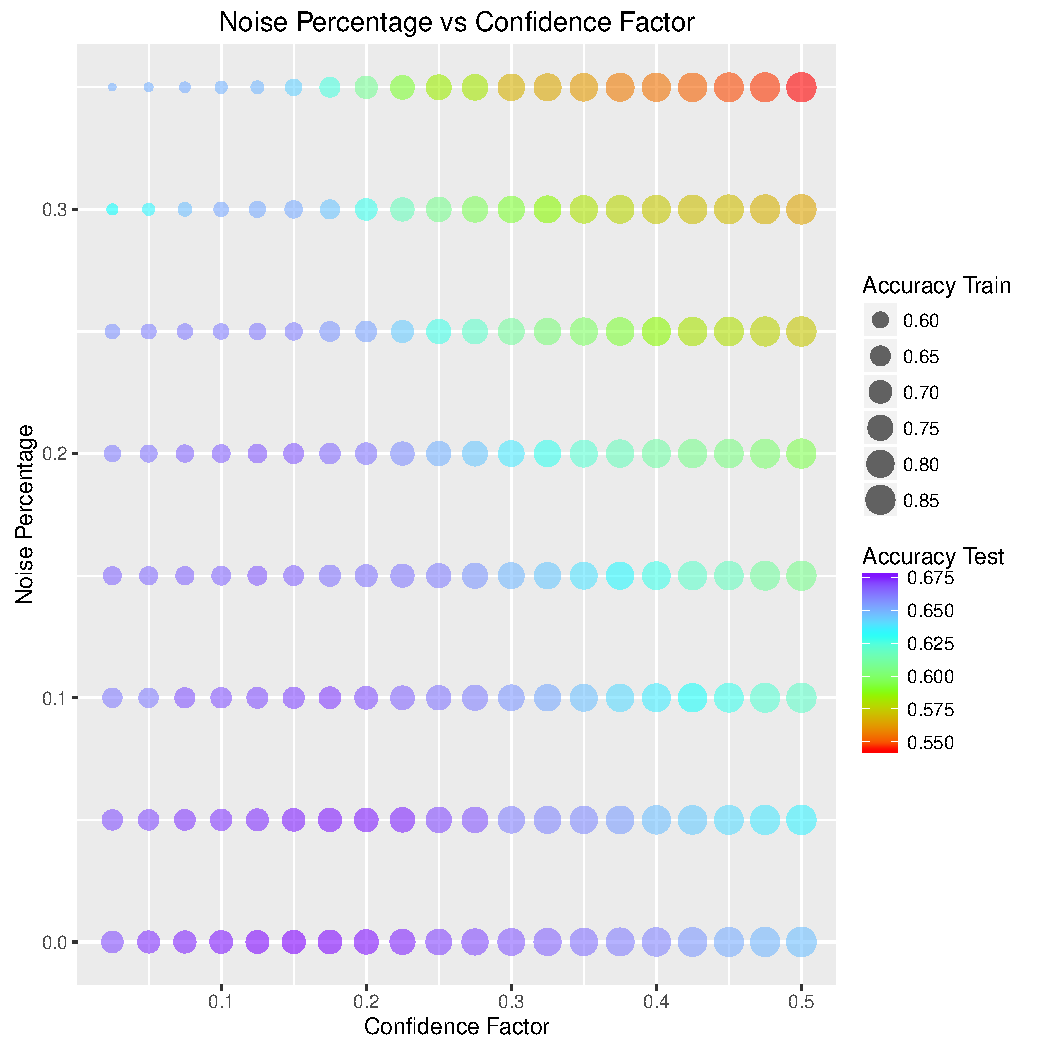
\includegraphics[width = 8cm]{5d.pdf}
  \caption{Noise percentage vs Confidence factor}
  \label{fig:5d}
\end{figure}

En la figura~\ref{fig:6a} se muestra la grafica de la curva ROC para el mejor árbol,

\begin{figure}
  \centering
  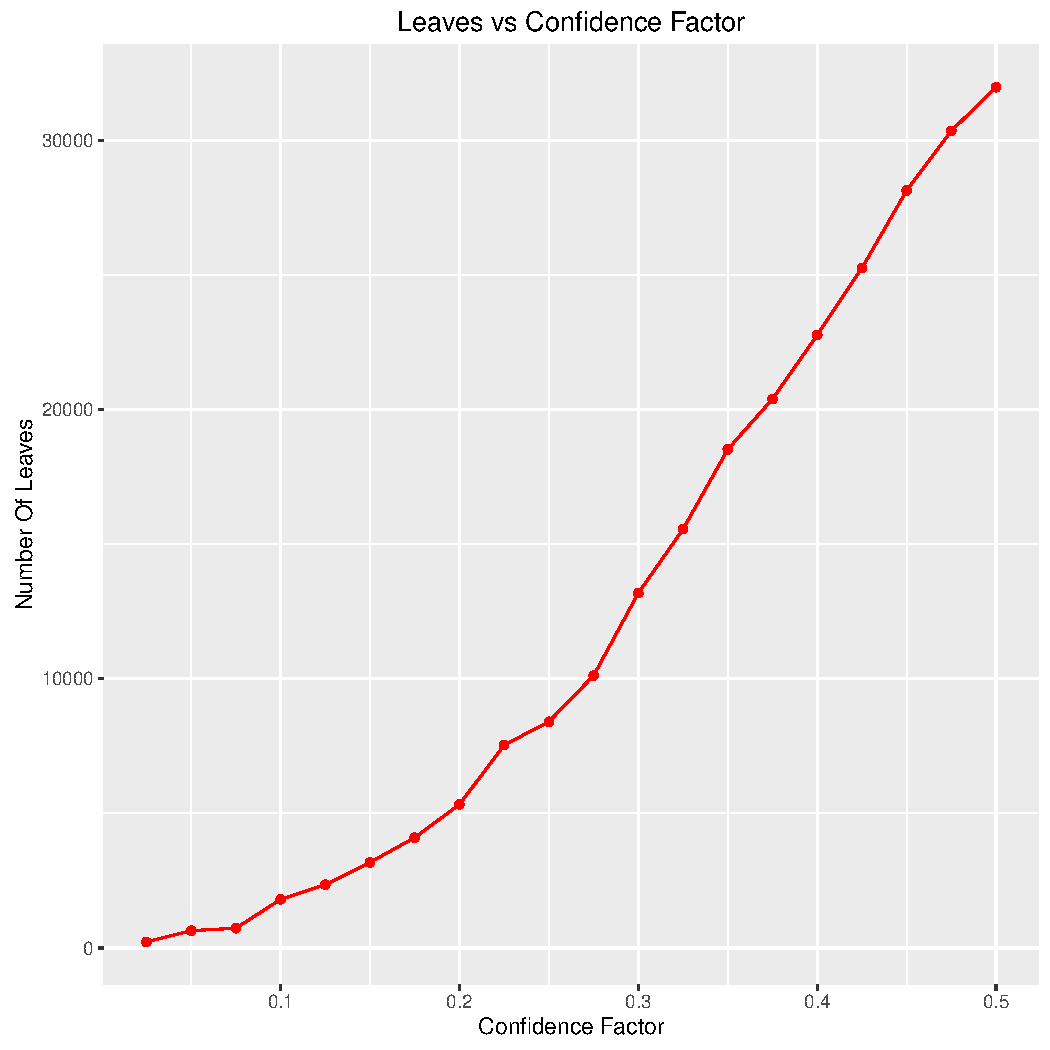
\includegraphics[width = 8cm]{6a.pdf}
  \caption{Number of leaves vs Confidence factor with supervised discretize}
  \label{fig:6a}
\end{figure}

En la figura~\ref{fig:6b} se muestra la grafica de la curva ROC para el mejor árbol,

\begin{figure}
  \centering
  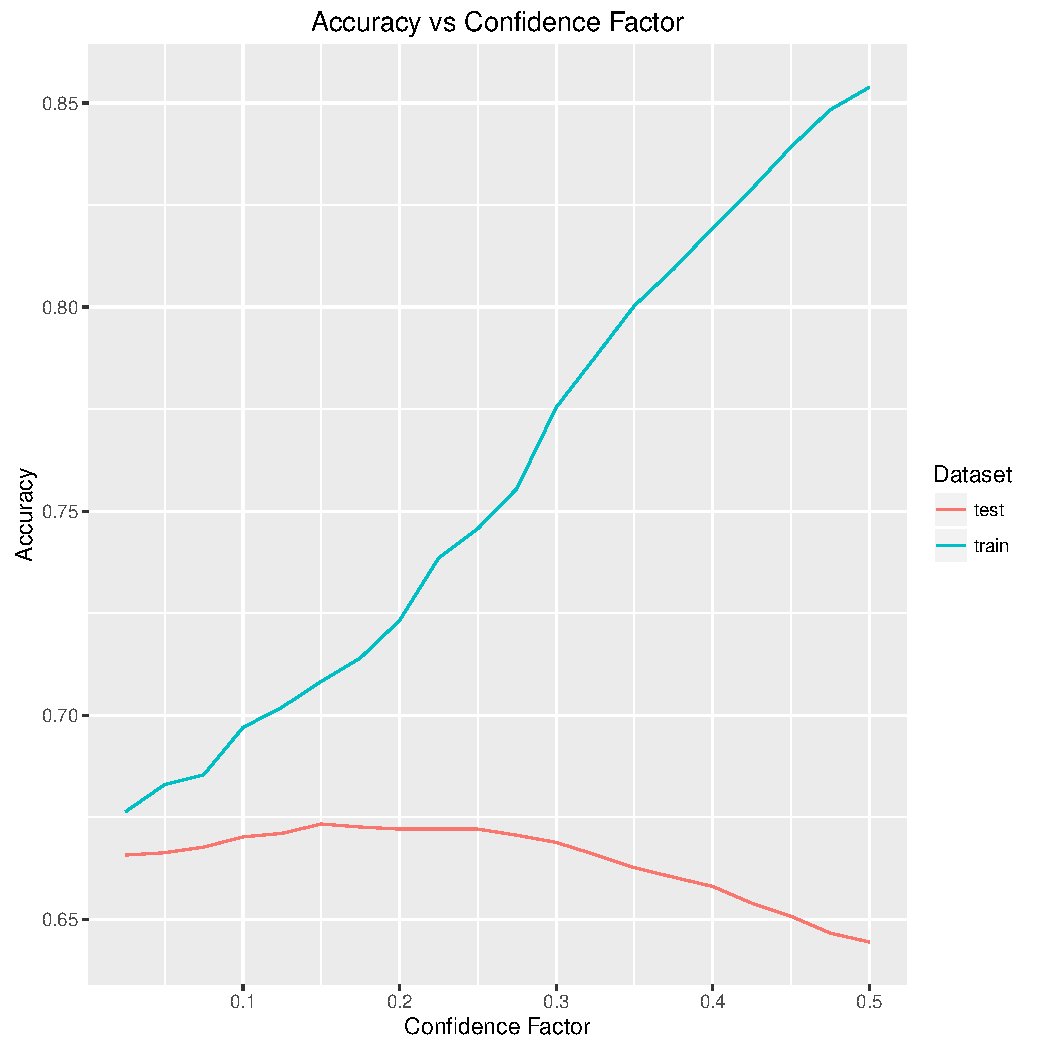
\includegraphics[width = 8cm]{6b.pdf}
  \caption{Accuracy vs Confidence factor with supervised discretized}
  \label{fig:6b}
\end{figure}

En la figura~\ref{fig:6c} se muestra la grafica de la curva ROC para el mejor árbol,

\begin{figure}
  \centering
  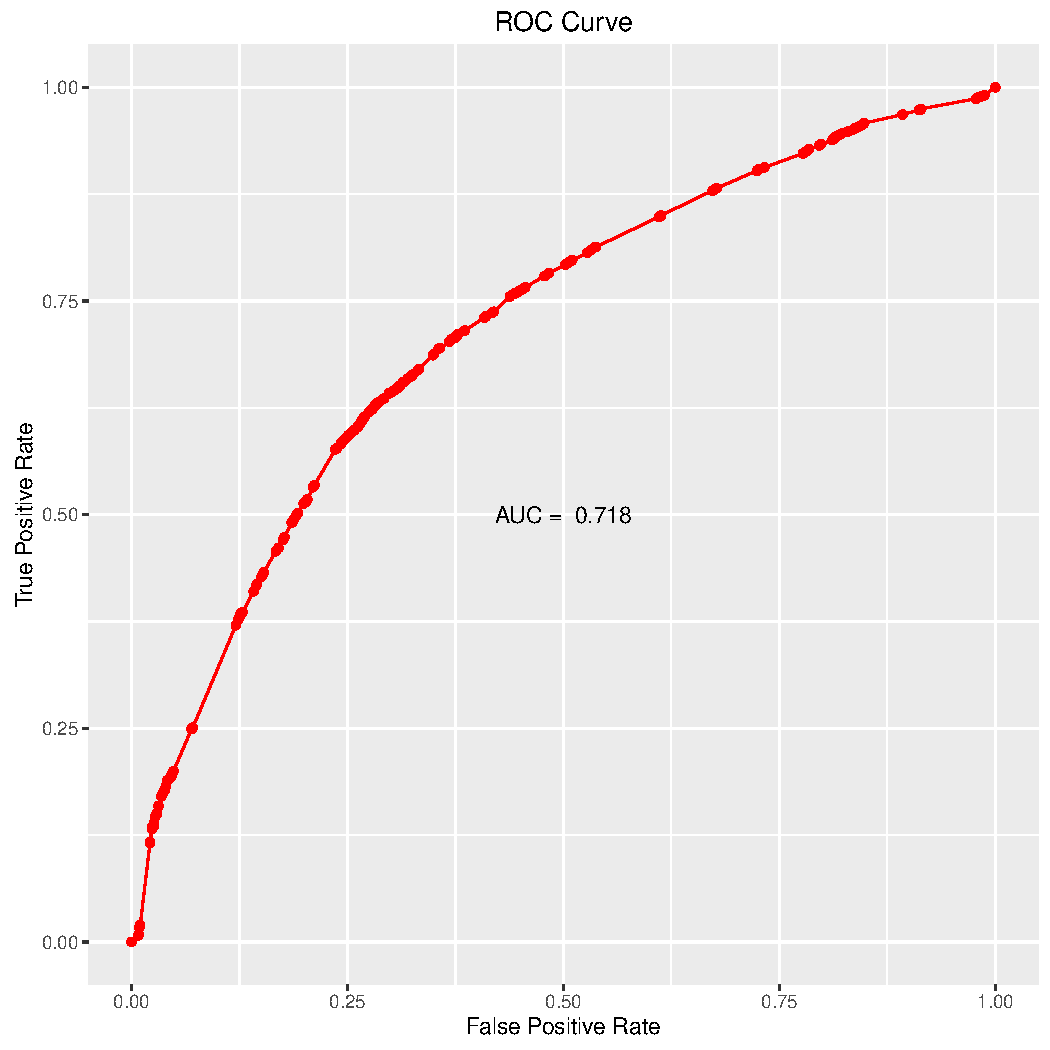
\includegraphics[width = 8cm]{6c.pdf}
  \caption{Curva ROC mejor árbol with supervised discretized}
  \label{fig:6c}
\end{figure}

En la figura~\ref{fig:6d} se muestra la grafica de la curva ROC para el mejor árbol,

\begin{figure}
  \centering
  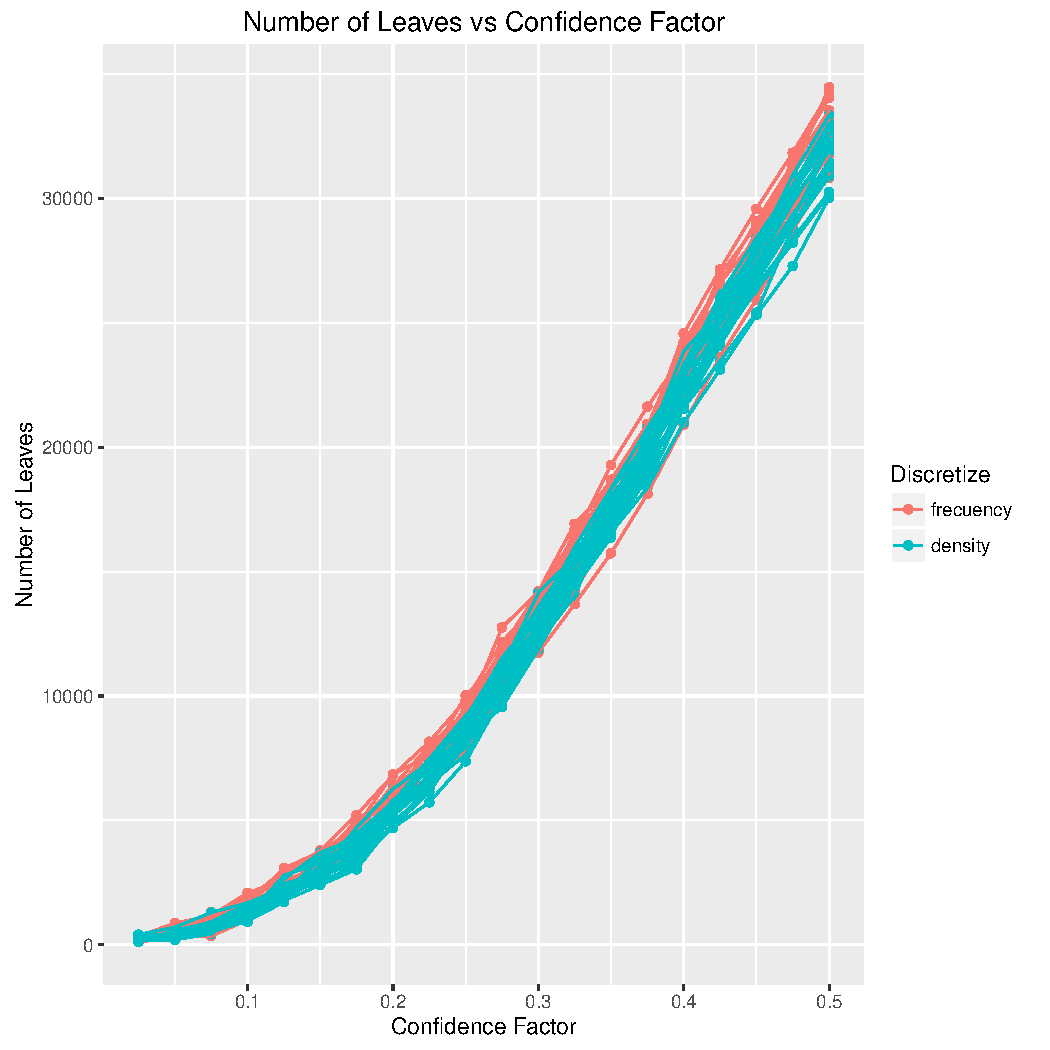
\includegraphics[width = 8cm]{6d.pdf}
  \caption{Leaves vs missing percentage with discretize}
  \label{fig:6d}
\end{figure}

En la figura~\ref{fig:6e} se muestra la grafica de la curva ROC para el mejor árbol,

\begin{figure}
  \centering
  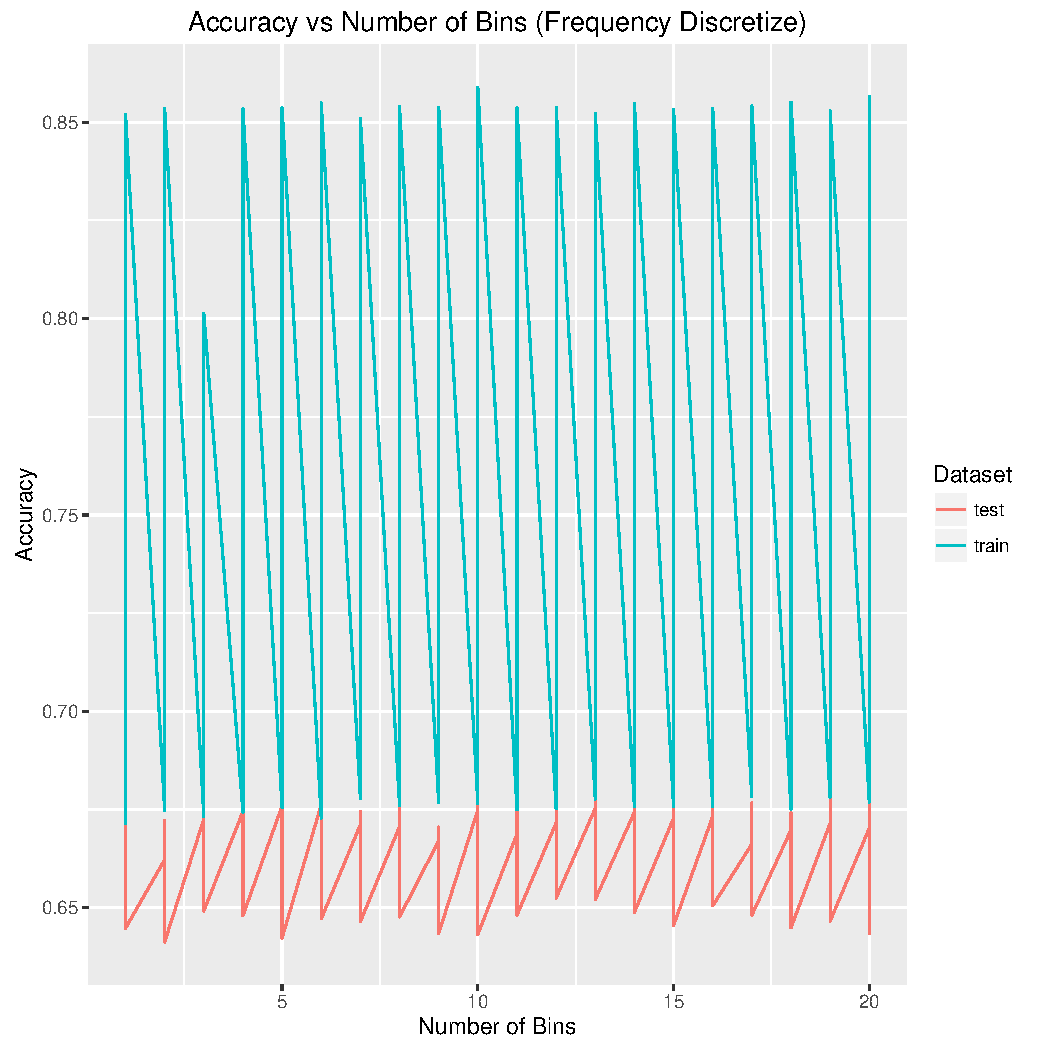
\includegraphics[width = 8cm]{6e.pdf}
  \caption{Accuracy vs Number of bins (Frequency discretize)}
  \label{fig:6e}
\end{figure}

En la figura~\ref{fig:6f} se muestra la grafica de la curva ROC para el mejor árbol,

\begin{figure}
  \centering
  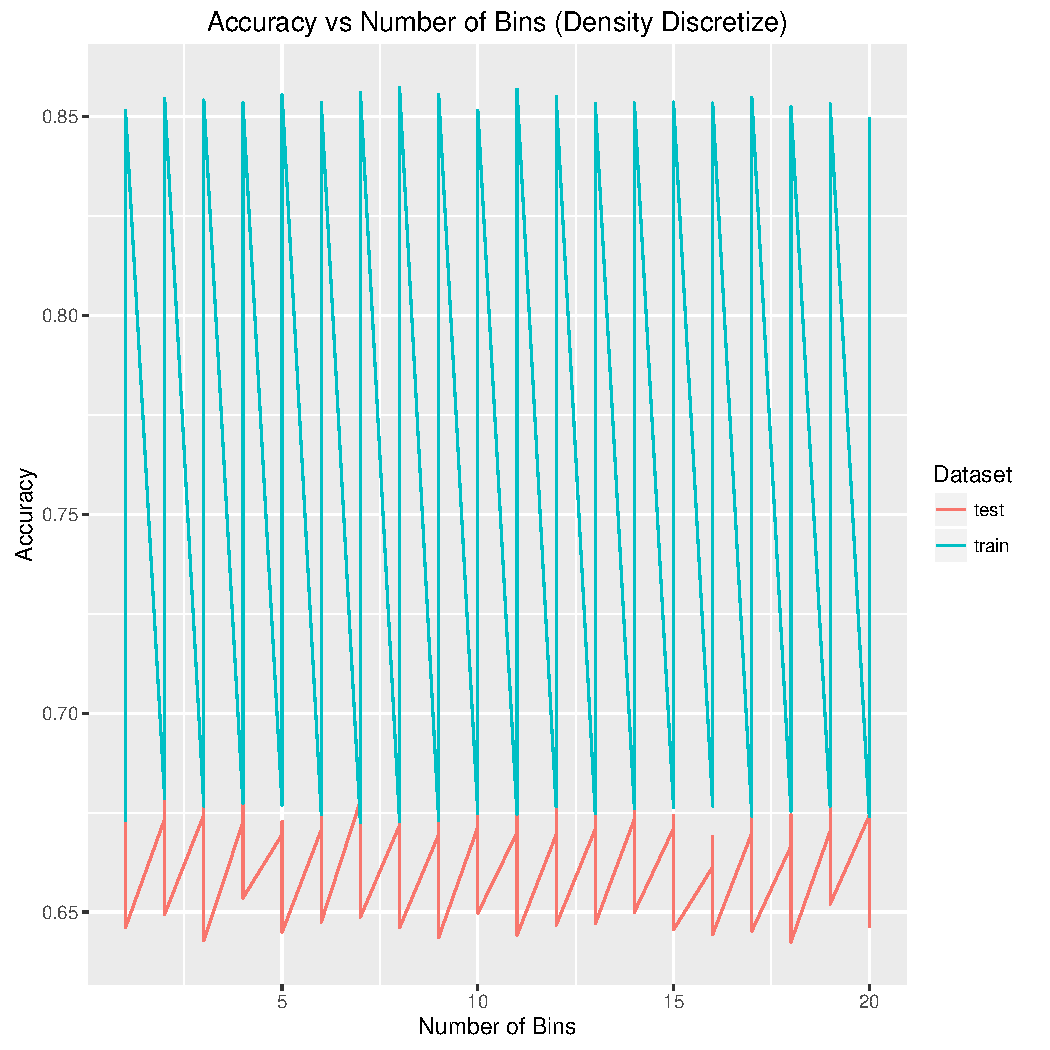
\includegraphics[width = 8cm]{6f.pdf}
  \caption{Accuracy vs Number of bins (Density discretize)}
  \label{fig:6f}
\end{figure}




